\documentclass{standalone}
\usepackage{tikz}
\usepackage{ctex,siunitx}
\setCJKmainfont{Noto Serif CJK SC}
\usepackage{tkz-euclide}
\usepackage{amsmath}
\usetikzlibrary{patterns, calc,3d}
\usetikzlibrary {decorations.pathmorphing,decorations.pathreplacing,decorations.shapes}
\tikzset{label style/.append style={font=\small}}
\begin{document}
\small
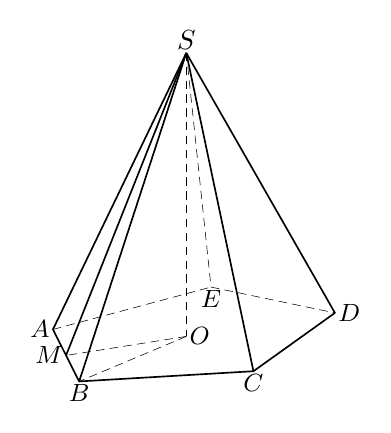
\begin{tikzpicture}[>=latex,scale=1.2,inner sep=1pt]
  \begin{scope}[z={(45:5mm)},canvas is zx plane at y=0]
    \foreach \x[count=\i from 0] in {E,D,C,B,A}
    {\tkzDefPoint(\i*72-10:1.5){\x}}
    \tkzDefPoints{0/0/O}
    \tkzInterLL(O,D)(A,B)\tkzGetPoint{M}
    \tkzDefMidPoint(A,D)\tkzGetPoint{O'}
    \tkzDefPointsBy[projection=onto A--D](B,C){G',H'}
    \tkzDrawSegments[semithick](A,B B,C C,D)
    \tkzDrawSegments[densely dashed](O,M O,B A,E E,D)
    \tkzLabelPoints(B,C,E)
    \tkzLabelPoints[right](D,O)
    \tkzLabelPoints[left](A,M)
  \end{scope}
  \draw[semithick](0,3,0)node[above]{$S$}--(A);
  \draw[very thin,densely dashed](0,3,0)--(E);
  \draw[very thin,densely dashed](0,3,0)--(O);
  \draw[semithick](0,3,0)--(B);
  \draw[semithick](0,3,0)--(M);
  \draw[semithick](0,3,0)--(C);
  \draw[semithick](0,3,0)--(D);
\end{tikzpicture}
\end{document}